\documentclass{article}
\usepackage[utf8]{inputenc}
\usepackage[T1]{fontenc}
\usepackage{geometry}
\usepackage{enumitem}
\usepackage{graphicx}

\geometry{margin=0.75in}

\begin{document}

\title{\textbf{Functional specification}
\\ \large{\textit{Ganics}}}
\author{\textbf{Adrian Chmiel}}
\date{4th June 2024}
\maketitle

\section{Project's goal}
The aim of the project is to utilize GAN networks for generating images with translated style. The program offers two possible style conversion modes:
\begin{enumerate}[label=\arabic*.]
    \setlength\itemsep{0pt}
    \item \textbf{Vincent Van Gogh Art} - images will resemble the artworks of Vincent Van Gogh
    \item \textbf{Cartoon} - images will resemble pictures from cartoons (or comics)
\end{enumerate}

\section{General information}
The program was written in Python 3.10. It uses the following libraries:
\begin{itemize}
    \setlength\itemsep{0pt}
    \item \textbf{matplotlib} - for creating plots and visualizing data
    \item \textbf{numpy} - for matrix operations
    \item \textbf{opencv-python} - for image processing
    \item \textbf{pandas} - for data analysis
    \item \textbf{pillow} - for image processing
    \item \textbf{pydot} - for visualizing model structure
    \item \textbf{tensorflow} - for creating and training GAN models
    \item \textbf{tkinter} - for creating a simple graphical interface
    \item \textbf{tqdm} - for displaying progress in model training
\end{itemize}

\section{Launching the program}
The program can be launched in several ways. One of the options is to use the available \textbf{\textit{ganics.exe}} file.
In case we would like to run the application directly from the source code, it is recommended to create a new virtual environment and install the required libraries in it.
Assuming that we are using \textit{conda}, we can do this with the following commands:
\begin{verbatim}
conda create -n Ganics python=3.10 -y
conda activate Ganics
conda install jupyter
pip install -r requirements.txt
\end{verbatim}
The installation of Jupyter can be skipped if we do not plan to use notebooks.
\vspace{3mm} \\
For NVIDIA graphics card owners, it is also worth running the following command, which will enable the use of CUDA:
\begin{verbatim}
conda install -c conda-forge cudatoolkit=11.2 cudnn=8.1.0 -y
\end{verbatim}
The program can be launched by calling the \textbf{\textit{main.py}} file:
\begin{verbatim}
python src/main.py
\end{verbatim}

\section{Graphical interface}
The graphical interface of the program was created using the \textit{tkinter} library. It allows:
\begin{itemize}
    \setlength\itemsep{0pt}
    \item Selection of the input file
    \item Selection of the conversion style
    \item Converting and saving the image
    \item Preview of the image before and after conversion
\end{itemize}
A sample screenshot of the graphical interface is shown below:
\vspace{3mm} \\
\includegraphics[width=0.5\textwidth]{../imgs/gui.png}

\section{Input and output files}
\begin{enumerate}[label=\arabic*.]
    \item \textbf{Main application} \\
The program allows selecting the path to the input file that will be converted. It is worth noting that the input file must be an image in the \textit{.jpg}, \textit{.jpeg}, or \textit{.png} format.
\vspace{3mm} \\
The output file, regardless of the initial format, is always an image in the \textit{.png} format with a resolution of \textit{512x512}.
    \item \textbf{Notebooks} \\
When it comes to notebooks, we provide entire sets of images as input (more information below), which will be used to train the model. As output, we receive visualizations illustrating how the model performs after training and an exported model weights file, which is later used as a component of the main application.
\end{enumerate}

\section{How the application works}
The application's operation concept is visible below:
\begin{enumerate}[label=\arabic*.]
    \item File selection and conversion style
    \item Image style translation using \textbf{CycleGAN} \\
\textit{The resulting image has a resolution of 256x256.}
    \item Image upscaling using \textbf{PatchGAN} to a resolution of 512x512
    \item Saving the image in the \textit{.png} format
\end{enumerate}
Important fact is that the application \textbf{will not work} if it does not find the appropriate model weights, which the user will be informed about by an error.
In such a case, it is necessary to either run the notebooks to train the model, or download the ready-made files available on \textit{Google Drive} under the link in the \textit{how\_to\_get\_models.md} file.

\section{Theory}
The program is based on two GAN network models:
\begin{itemize}
    \setlength\itemsep{0pt}
    \item \textbf{CycleGAN}
    \item \textbf{PatchGAN}
\end{itemize}
\textbf{GAN} \textit{(Generative Adversarial Network)} is a type of artificial neural network that consists of two models: \textbf{generator} and \textbf{discriminator}.
The generator's task is to generate new images that are similar to those from the dataset, while the discriminator's task is to distinguish whether the image comes from the generator or the dataset.
The training process involves a competition between both models, where the generator tries to deceive the discriminator, and the discriminator tries to learn to distinguish images.
As a result, the generator is able to generate images very similar to those from the dataset.
\vspace{3mm} \\
More information about the operation of these models is available in the document: \textit{Note\_about\_GANs.pdf}

\section{Datasets}
To obtain datasets for training models, you can extract the available \textit{.zip} files, which contain images selected by me from the datasets listed below. An alternative option is to use the links to these datasets available in the \textit{README.md} file. This approach will allow you to independently choose images that will be used for training.
\vspace{3mm} \\
The datasets used for training models are:
\begin{itemize}
    \item \textbf{Familyguy} (from the Cartoon Classification dataset) \\
Used to train CycleGAN responsible for converting the style to a cartoon (or comic).
    \item \textbf{VincentVanGogh} (from the Vincent Van Gogh Art dataset) \\
Used to train another CycleGAN responsible for converting the style to Vincent Van Gogh's artworks.
    \item \textbf{natural\_images} \\
Sample images, the style of which was transformed into one of the two mentioned above during training.
    \item \textbf{mscoco} \\
A dataset that additionally expanded the set of data with natural images used to train the models.
\end{itemize}

\section{Limitations}
Style conversion is a relatively complex task, so the training time in notebooks strongly depends on the computational power of the computer. For this reason, it is recommended to use an NVIDIA graphics card, which significantly speeds up the learning process. All notebooks are adapted to use CUDA if available, that is the required software has been installed.
\vspace{3mm} \\
It is also worth noting that the cartoon style is relatively simple, so the model will cut off the details of the images during conversion. In the case of too complex images, the result may be unsatisfactory.

\section{Visualization of featured models}
On the following pages, visualizations of the models used in the application are visible. These visualizations were generated using the \textit{pydot} library. They show both the generator and the discriminator for both models, along with individual layers and their connections. More information is available in the documents:
\begin{itemize}
    \setlength\itemsep{0pt}
    \item \textit{Note\_about\_GANs.pdf}
    \item \textit{Note\_about\_layers.pdf}
\end{itemize}
\newpage
\begin{enumerate}[label=\arabic*.]
    \item \textbf{CycleGAN - Generator}
        \vspace{3mm} \\
        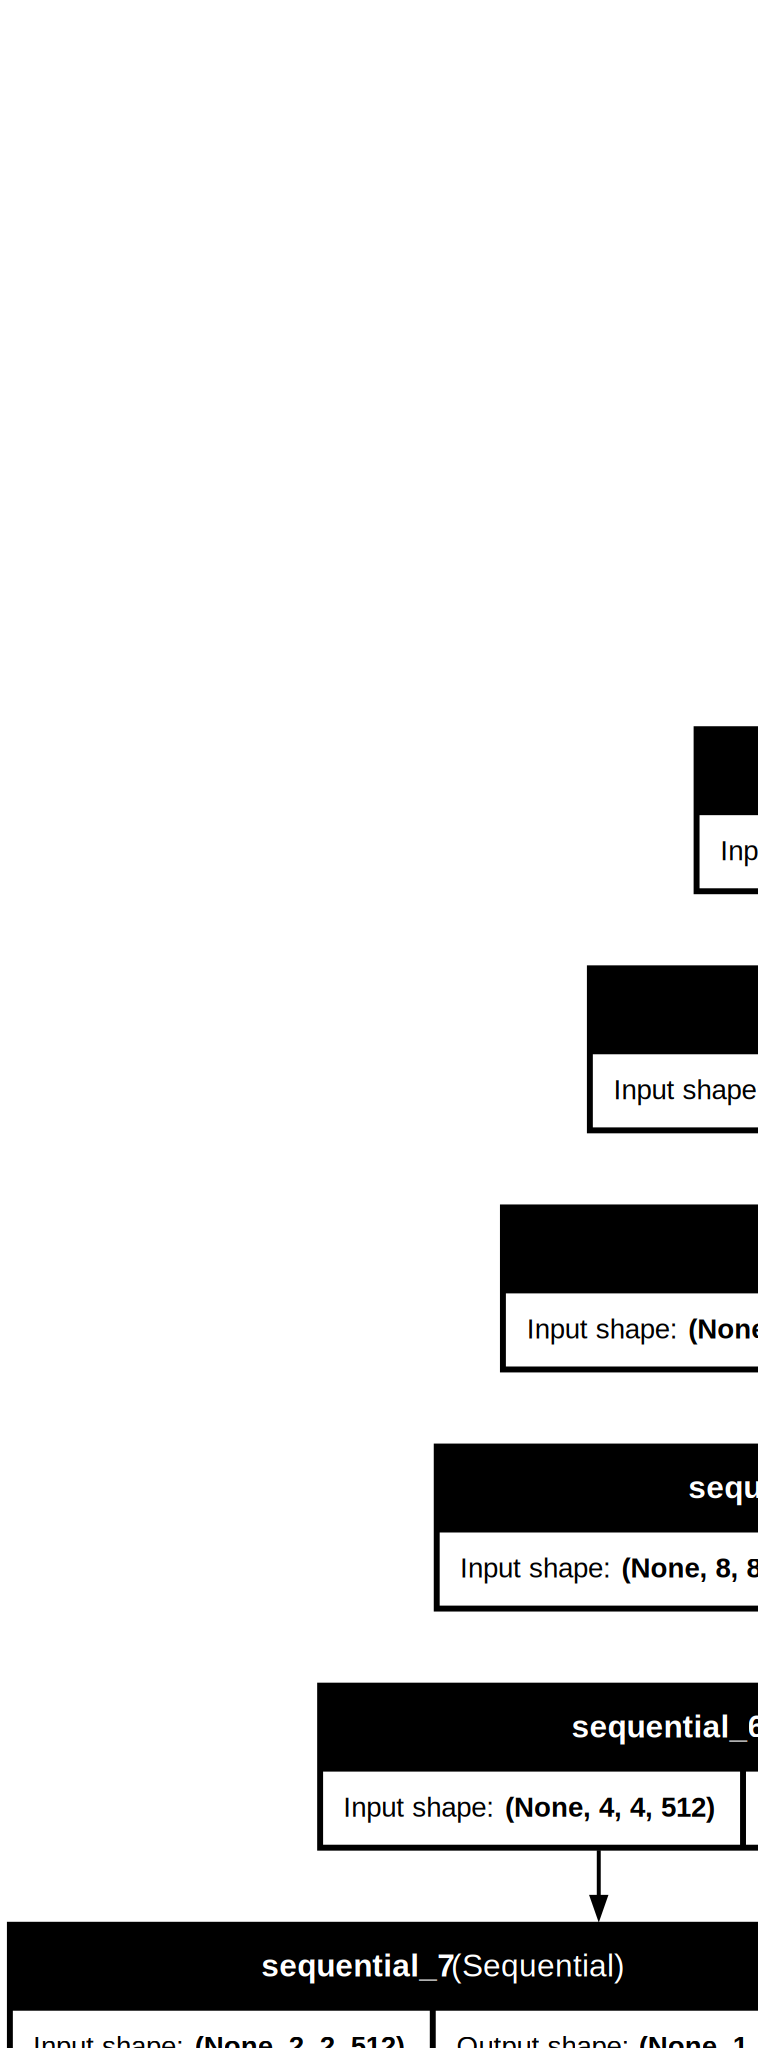
\includegraphics[height=0.95\textheight]{../imgs/cyclegan_generator.png}
        \newpage
    \item \textbf{CycleGAN - Discriminator}
        \vspace{3mm} \\
        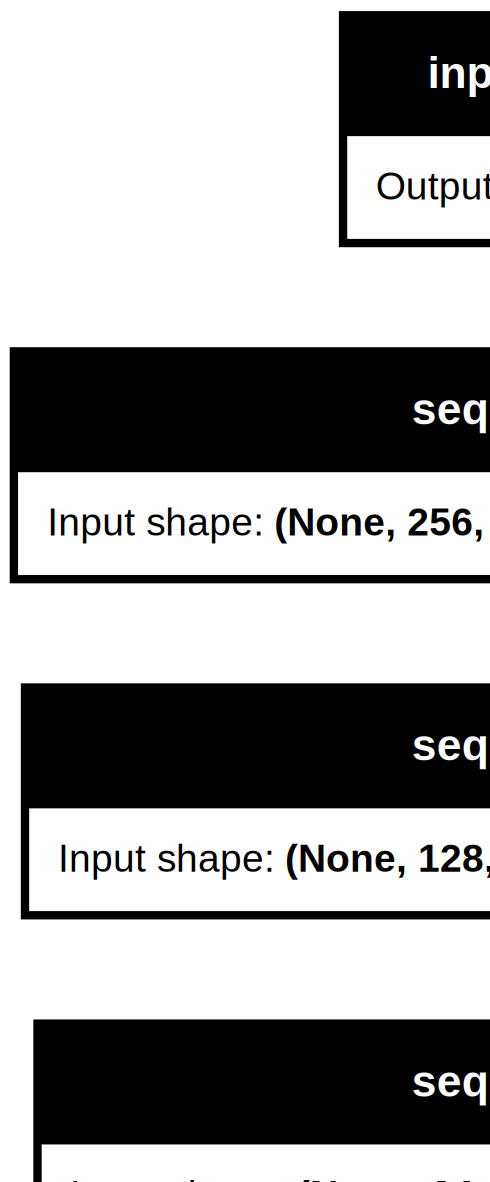
\includegraphics[height=0.95\textheight]{../imgs/cyclegan_discriminator.png}
        \newpage
    \item \textbf{PatchGAN - Generator}
        \vspace{3mm} \\
        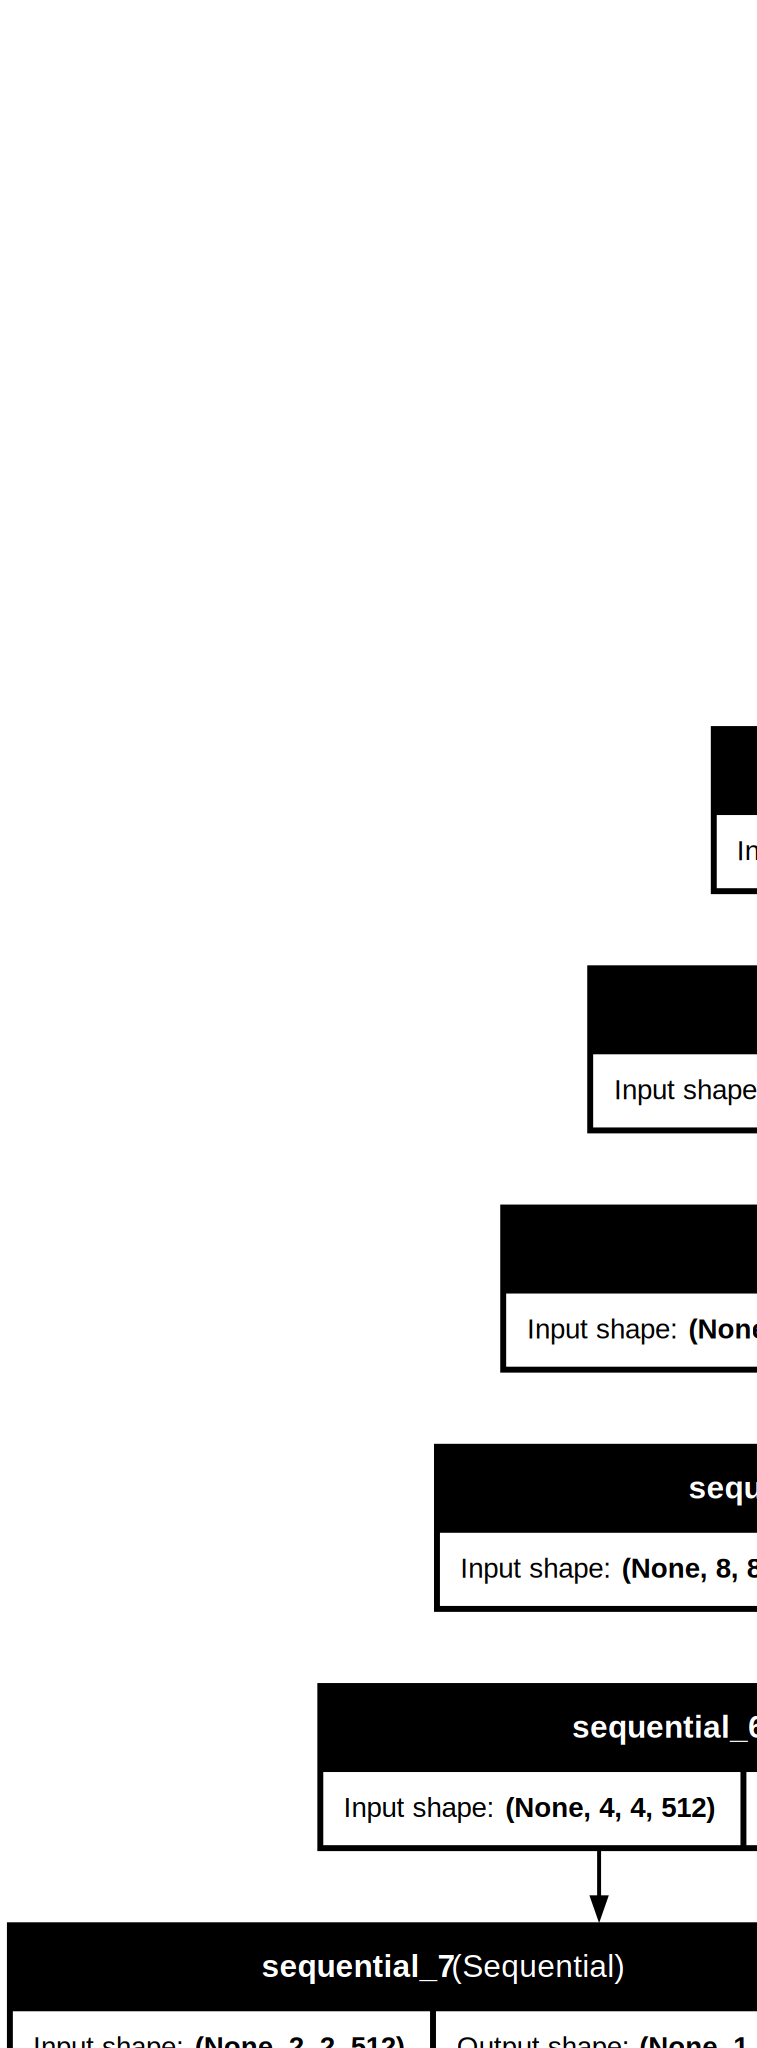
\includegraphics[height=0.95\textheight]{../imgs/patchgan_generator.png}
        \newpage
    \item \textbf{PatchGAN - Discriminator}
        \vspace{3mm} \\
        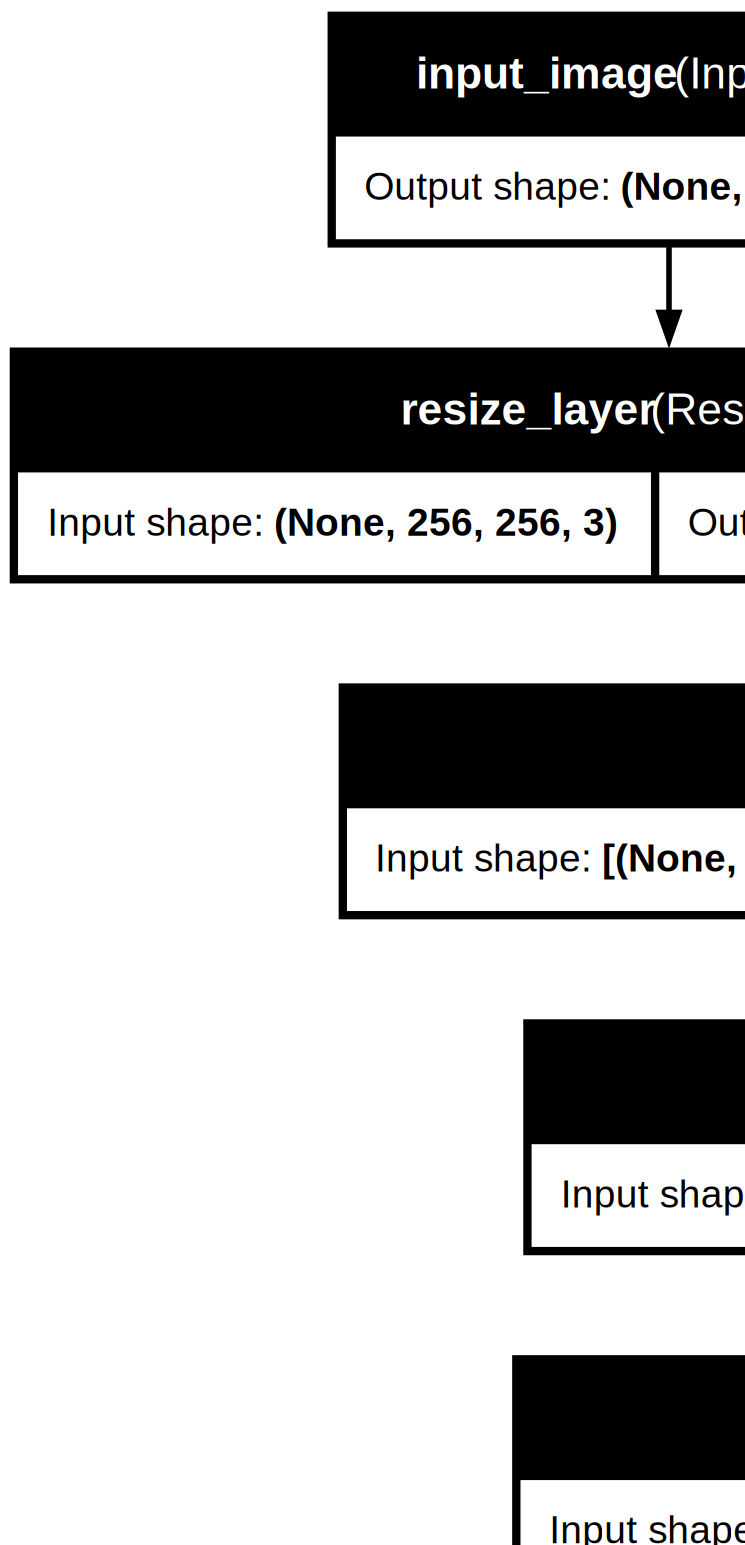
\includegraphics[height=0.95\textheight]{../imgs/patchgan_discriminator.png}
        \newpage
\end{enumerate}

\end{document}